%Chapter describing the model
\chapter{Modeling the evolution of mimicry}

\section{Past Work}

\subsection{Sherratt's Model}

\subsection{Models by Frank and Noble}

\section{FormAL Framework}

\subsection{Spatial representation of the environment}

\subsection{3D Visualization}

\subsection{Agents}

\subsection{Mobility}

\section{Mimics and Model}

\subsection{Pattern representation by Cellular Automata}

\subsection{Species diversity}

\subsection{Genetic representation of palatability}
The palatability of each prey species is fixed and has been represented with 2 bit of the genome giving it a range of 0 to 3 with four levels of palatability. The combinations are as follows:

\begin{table}[H]
	\centering
	\begin{tabular}{|c|c|}
		\hline
			Gene (Index 8 to 9) &	Palatable \\ \hline
			00									& True 			\\ \hline
			01									& True 			\\ \hline
			10									& False 		\\ \hline
			11									& False 		\\
		\hline
	\end{tabular}
	\caption{Genetic representation of Palatability}
	\label{tab:genetic-representation-palatability}
\end{table}

This representation in Table \ref{tab:genetic-representation-palatability} is unlike \cite{franks2003} where palatability level has been used on a scale between zero and one (least to most palatable), where 0.5 is neutrally palatable. 

\subsection{Interaction between Mimics and Models}

\subsection{Interaction with predators}

\section{Predator}

\subsection{Learning}

\subsubsection{Hebbian Learning}

\subsection{Design of Memory with Hopfield Network}

\subsubsection{Hopfield Network}

\subsection{Genetic representation of mobility and reproduction capability}
Each predator in the simulation has a genetic representation. The genome of the predator is represented with a 5 bits binary value. 

\begin{table}[H]
	\centering
	\begin{tabular}{|c|c|c|c|c|}
		\hline
			\multicolumn{4}{|c|}{Mobility} &	Reproduction Capability \\ \hline
			1	& 0 &	1	& 0 								&	1\\
		\hline
	\end{tabular}
	\caption{Genetic representation of Mobility and Reproduction capability}
	\label{tab:genetic-representation-mobility-reproduction}
\end{table}

Movement behavior of a Predator calculated from its Genome. The first 4 bits of the genome of this species are converted from binary to decimal to determine the magnitude of force at which it will move towards the maximum crowd of Prey present within its neighborhood. So mobility of a predator varies within a range of 0-15 units. If no prey is present in the neighborhood then this force is active in trying to keep predators distributed all over the cells. A predator chooses the neighborhood cell which contains the least number of predators. When the neighborhood contains zero predators, it would select any one of them randomly and move towards that cell.

\begin{figure}[H]
	\centering
	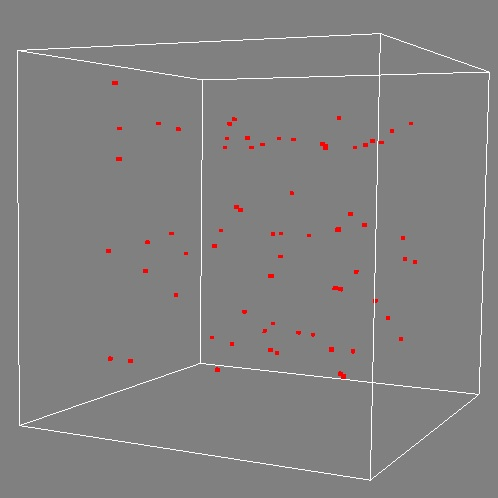
\includegraphics[scale=0.40]{images/predators-40}
	\caption{A population of 40 predators distributed over the environment.}
	\label{fig:predators-40}
\end{figure}

The screen shot in Figure \ref{fig:predators-40} is from the simulation with only 40 predator species. It is presented to show the behavior of predator species in the simulation in absence of any prey species. As it can be observed the predator are distributed all over the cells with a constant mobile behavior to switch to another neighboring cell depending on which ever contains the least number of predator and also most number of prey species. This behavior of predator has been designed to enforce the predatory behavior of this species and also to have increase predator prey interaction in the simulation in terms of one species chasing the other for search of food. 

The  fifth gene of the predator is used to represent their capability of reproduction.  Depending on its binary value a predator in the simulation will or will not be able to reproduce in the simulation. 

\subsection{Reproduction process}
The reproduction process for predators is similar to prey species. As the learning capability of predators do not have any genetic representation, only the mobility behavior and reproduction capability behavior takes effect in the reproductive process of predator species from one generation to another. 

There are two control parameters that effect reproduction of predator species in the simulation. The first is the "Reproduction Age Limit". This the minimum age a predator has to reach before starting to involve itself for reproduction. This parameter has been set to 500 iterations during the result and analysis section of the thesis. The second parameter is "Reproduction Interval" which has been varied in the simulation from 1000 to 3000 iteration depending on the population of palatability of the prey species. This is a very important parameter for the simulation as it determines the overall predator population and its rate of increment. Depending on this value we can control the rate of predation on prey species, which on the other hand controls the rate of mimetic behavior of the overall prey population.

When the above two conditions are met, meaning the predator reaches it age for reproduction and also crosses every age interval, it randomly select another predator residing in the same cell. If this random predator is capable to reproduce depending on its 5th gene, then with a random single point crossover and mutation a new predator species in born which also resides on the same cell and initializes with zero memory configuration. Similarly when the new born predator reaches its maturity of reproductive age and if its capable to reproduce then the process iterates itself. 

\subsection{Interaction with Models and Mimics}